\documentclass[10pt, twocolumn]{article}
\usepackage[utf8]{inputenc}
\usepackage[mathscr]{euscript}
\usepackage{kpfonts}
\usepackage{commath}
\usepackage{amsthm}
\usepackage{graphicx}

\newcommand{\R}{\ensuremath{\mathbb{R}}}
\newcommand{\N}{\ensuremath{\mathbb{N}}}
\newcommand{\Q}{\ensuremath{\mathbb{Q}}}
\newcommand{\B}{\ensuremath{\mathcal{B}}}
\newcommand{\wrt}{with respect to}
\newcommand{\Iff}{if and only if}
\newcommand{\es}{\ensuremath{\emptyset}}
\newcommand{\script}[1]{\ensuremath{\mathscr{#1}}}
\newcommand{\coleq}{\ensuremath{\coloneqq}}
\newcommand{\powset}[1]{\ensuremath{\mathcal{P}(#1)}}
\newcommand{\define}[1]{\textbf{\underline{#1}}}
\newcommand{\func}[3]{\ensuremath{#1: #2 \to #3}}
\newcommand{\union}{\cup}
\newcommand{\Union}{\bigcup}
\newcommand{\inter}{\cap}
\newcommand{\Inter}{\bigcap}
\renewcommand{\Subset}{\subseteq}
\renewcommand{\Supset}{\supseteq}

\theoremstyle{definition}
\newtheorem*{defn}{Definition}
\newtheorem*{cor}{Corollary}
\newtheorem*{thm}{Theorem}
\newtheorem*{prop}{Proposition}
\newtheorem*{ex}{Ex}
\newtheorem*{lem}{Lemma}

\theoremstyle{remark}
\newtheorem*{rmk}{Remark}

\begin{document}
    \begin{titlepage}
        \begin{center}
            \vspace*{1cm}
                
            \Huge
            \textbf{Bookshelf Modeling}
            
            \vspace{0.5cm}
            \Large 12 May 2021
                
            \vspace{1.5cm}
                
            \textbf{Dillan Marroquin}
                
            \vfill
            
            \large
            MATH 305.1001\\
            Dr. Keppelmann \& Dr. Waddell\\
            University of Nevada, Reno\\
        \end{center}
    \end{titlepage}
    
    \subsection*{\textsc{Problem and Sampling Method}}{
        The goal of this paper is to give an accurate estimate of the number of pages in Professor Waddell's really big bookshelf (see Figure 4). He is clearly very well read! 
        
        Although we discussed a few different sampling methods during lecture (SRS, Cluster, and Stratified), we will be conducting a cluster sample. There were two reasons why cluster sample was chosen as our sampling method: 1) Glenn's bookshelf can easily be divided into different clusters using each shelf as a cluster and 2) most of the shelves are very heterogeneous in the sense that the sub-populations (the books on each shelf) are very representative of the entire population (the books in the bookcase). We use the $17$ shelves of the bookshelf as our clusters. First, we assign each shelf a number from $1$-$17$, where Shelf $1$ is the top-left shelf, and Shelf $17$ is the bottom-right shelf. Since we are only interested in the shelves that best represent the population of interest, we exclude shelves $13,14,15,16,$ and $17$ from our sampling frame since the books in these shelves are all very homogeneous. Next, we perform an SRS to choose Shelf $4$ as our sample and then take a census to discover the number of pages in each book and the width of each book in Shelf $4$.
    }
    \subsection*{\textsc{Assumptions and Variables}}{
        Next, we make a few assumptions that are important for our calculations. First, we assume a "page" to be a single piece of paper, front and back. This implies that a book's page count is actually double the number of pages we desire. Second, we assume that a book's cover is not considered a page. These assumptions ensure that our calculations are clearly defined and consistent. Lastly, we assume that page thickness can be ignored. This assumption is made because the difference in page thickness between books is likely negligible and thus should not significantly impact the final result.
        
        Our variables of interest for this experiment are the number of pages within a book, and book width. Using our intuition, we hypothesize that book width and the number of pages in a book are related. Other variables such as book height or page thickness were ignored since they were hypothesized to not significantly impact the final result
    }
    \subsection*{\textsc{Methods and Calculations}}{
        Using the data provided to us by Professor Waddell (Figure 1), we construct a scatter plot of book width vs book pages for each of the books on Shelf $4$.
        
        \begin{figure}[h]
            \centering
            \graphicspath{images}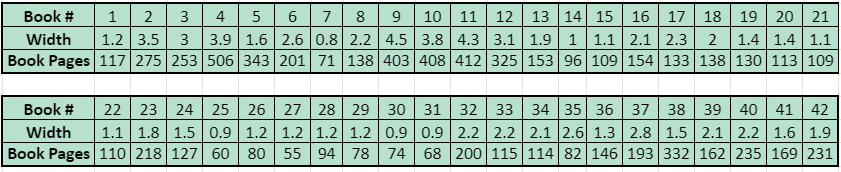
\includegraphics[width=9cm, height=2cm]{images/Table.png}
            \caption{Data collected by Professor Waddell}
        \end{figure}
        
        From the scatter plot (Figure 2), we can see that there is indeed a strong positive correlation between a book's width and its page count. Using the R software, we find the estimated $y$-intercept to be $-5.01$ and the estimated slope to be $93.03$. Using these calculations, we come up with a function for a book's pages, $P$, in terms of a book's width, $w$: $P(w)=93.03w-5.01$.

        \begin{figure}[h]
            \centering
            \graphicspath{images}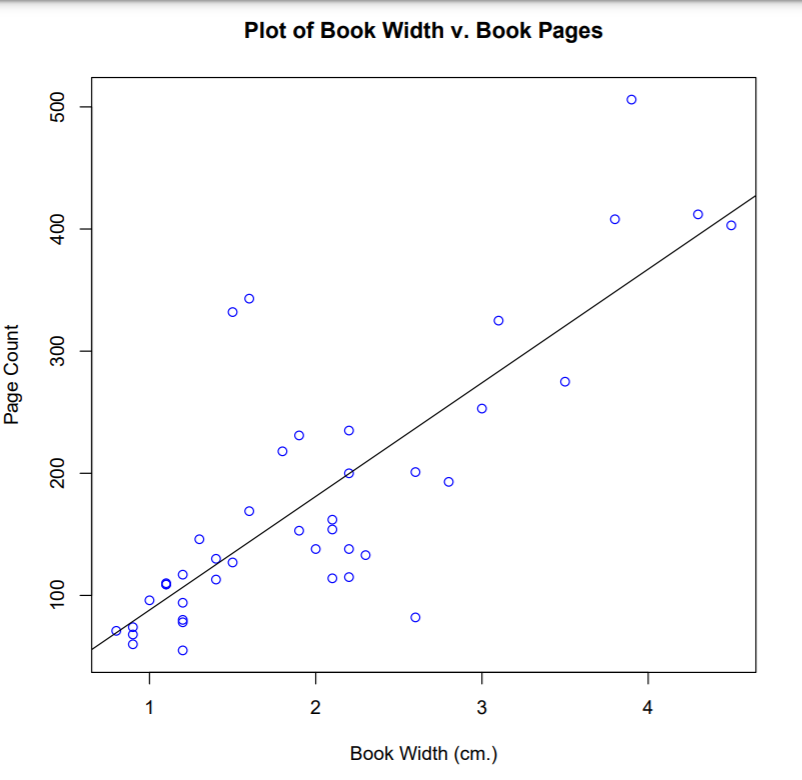
\includegraphics[width=5.5cm, height=4.1cm]{images/Scatterplot.png}
            \caption{Book Width v Book Pages Scatter-plot}
        \end{figure}
        
        As for the residual plot (Figure 3), we see that the plotted values are equally and randomly spaced about the horizontal axis, thus making this a good residual plot.
    
        \begin{figure}[h]
            \centering
            \graphicspath{images}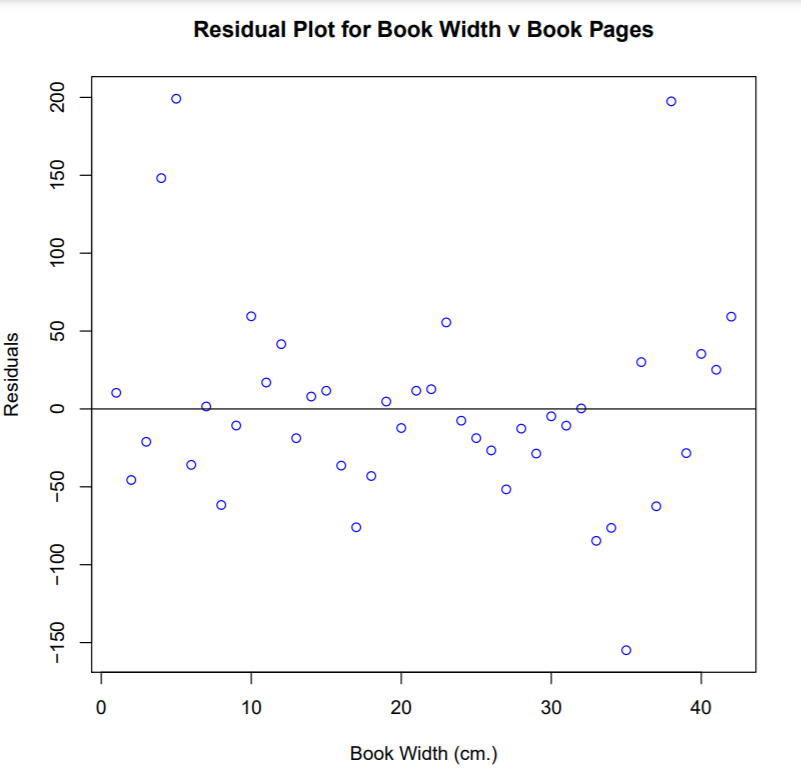
\includegraphics[width=5.5cm, height=4.1cm]{images/Residual Plot.png}
            \caption{Book Width v Residuals Residual Plot}
        \end{figure}    

        The total number of pages in Shelf $4$ is calculated to be $7530$ based on the information provided by Professor Waddell. Since Shelf $4$ is a good representation of the population, we can assume $7530$ is a good estimate for the number of pages in each individual shelf. By this logic, \textbf{there are approximately $\mathbf{7530(17)=128010}$ pages on Glenn's bookshelf.}
        
        However, we can do better. As mentioned previously, Shelves $13$-$17$ are very homogeneous, so we can expect the number of pages in these shelves to be different than the number of pages in Shelf $4$. Through some calculations, we find there are $32,37,28,28,$ and $34$ books on Shelves $13,14,15,16,$ and $17$ respectively. We also notice that Book $32$ from Shelf $4$ looks (at a glance) to have the most similar width of the books on Shelves $13$-$17$. Assuming that all the books on these shelves have the same page count as Book $32$ (200 pages), we can say that Shelves $13$-$17$ have $200(32+37+28+28)=31800$ pages. Using the same estimate as the previous method, we can say that there are approximately $7530(12)=90360$ pages on Shelves $1$-$12$. Thus \textbf{a better approximation of the number of pages on Glenn's bookshelf is $\mathbf{31800+90360=122160}$ pages.}
    }
        
    \subsection*{\textsc{Does the Result Make Sense?}}{
        This result makes logical sense. If we assumed each of the $42$ books in Shelf $4$ had the same number of pages as the book with the most pages (Book 4, 4.2 centimeters, 506 pages), our approximation for the number of pages in Glenn's bookshelf would be $17(42(506))=361284$. This is an outrageously large approximation which assumes that each book has a width of about $4.2$ centimeters; most books, unless they are textbooks or very large novels, will not be of this size.
        
        Inversely, if we assumed each book in Shelf $4$ had the same number of pages as the book with the least amount of pages (Book 27, 1.2 centimeters, 55 pages), our approximation for the number of pages in Glenn's bookshelf would be incredibly low at $17(42(55))=39270$. Just from observing the picture of Glenn's bookshelf, we can see why this is incorrect: hardly any books are as thin as 1.2 centimeters. Thus by looking at both the upper and lower bounds of the bookcase based off the data from Shelf $4$, we can safely say our result makes sense. 
        
        \begin{figure}[h]
            \centering
            \graphicspath{images}\includegraphics[width=8cm, height=7cm]{images/Bookshelves.jpg}
            \caption{ Professor Waddell's bookshelf. Just by observation, we can see our estimation of pages is well within the estimated upper and lower bounds}
        \end{figure}
    }
\end{document}